\section{Lezione 1}%
\label{sub:Lezione 1}
\marginpar{
    \captionsetup{type=figure}
    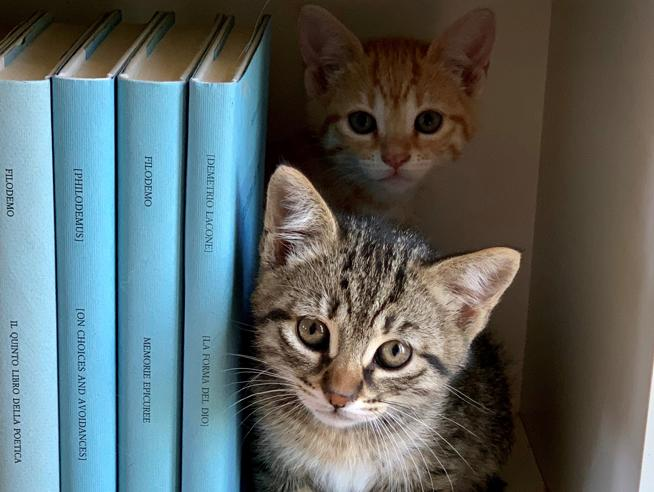
\includegraphics[width=\marginparwidth]{figures/cat.jpg}
    \caption{A cube represented as the 6 square faces that bound it}
    \label{fig:brep}
}

\marginpar{
    \captionsetup{type=figure}
    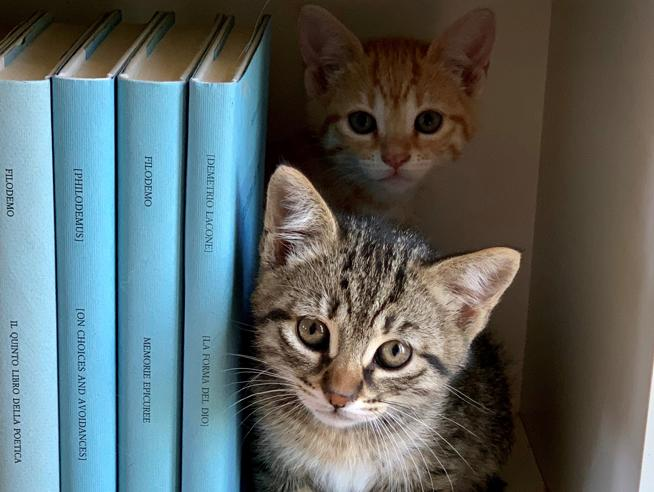
\includegraphics[width=\marginparwidth]{figures/cat.jpg}
    \caption{A cube represented as the 6 square faces that bound it}
    \label{fig:brep}
}
\marginpar{
    \captionsetup{type=figure}
    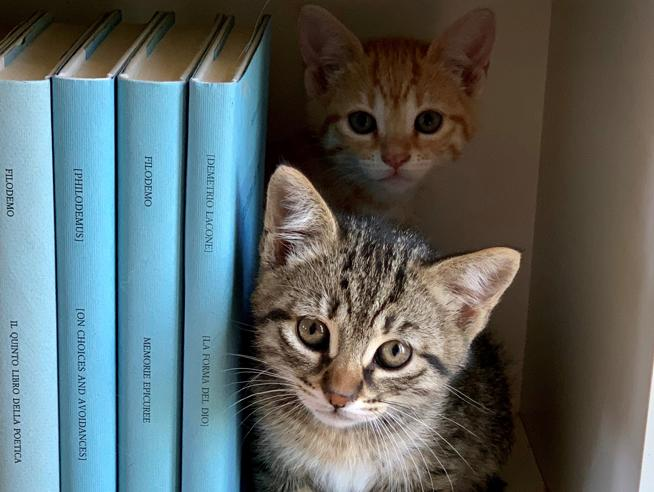
\includegraphics[width=\marginparwidth]{figures/cat.jpg}
    \caption{\scriptsize A cube represented as the 6 square faces that bound it}
    \label{fig:brep}
}
\marginpar{
    \captionsetup{type=figure}
    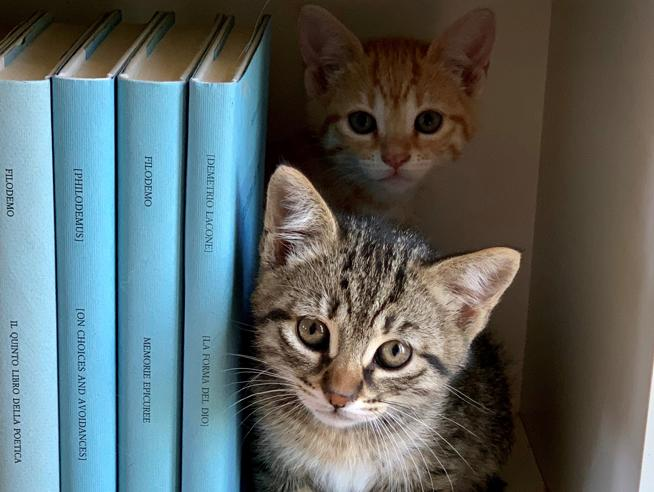
\includegraphics[width=\marginparwidth]{figures/cat.jpg}
    \caption{A cube represented as the 6 square faces that bound it}
    \label{fig:brep}
}
prova ciao ciao
\lipsum[2-6]

\marginpar{
    \captionsetup{type=figure}
    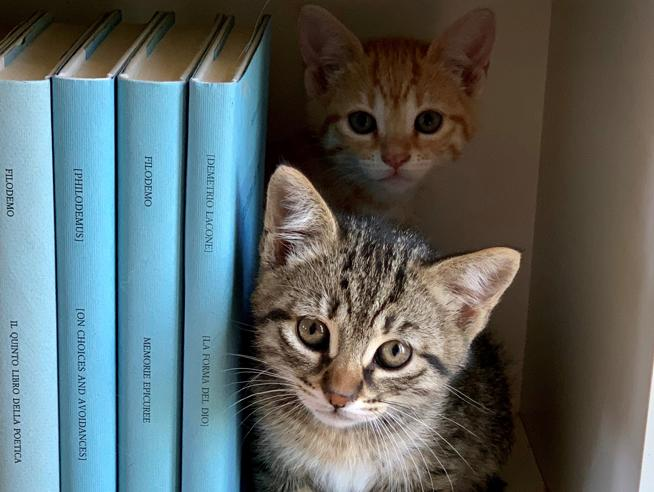
\includegraphics[width=\marginparwidth]{figures/cat.jpg}
    \caption{A cube represented as the 6 square faces that bound it}
    \label{fig:brep}
}
